\documentclass[11pt,a4paper]{article}

%---------------------------------------------------------------- page & fonts
\usepackage[a4paper,margin=2.5cm,headheight=14pt]{geometry}
\usepackage[T1]{fontenc}
\usepackage[utf8]{inputenc}
\usepackage{charter}                      % serif body: warmer than Computer Modern
\usepackage[scaled=0.92]{helvet}          % sans for headings
\usepackage{microtype}                    % subtle spacing/protrusion; big legibility win

%------------------------------------------------------------------- structure
\usepackage{amsmath}
\usepackage{graphicx}
\usepackage{booktabs}
\usepackage{array}
\usepackage{listings}
\usepackage{xcolor}
\usepackage{caption}
\usepackage{enumitem}
\usepackage{titlesec}
\usepackage{fancyhdr}
\usepackage{tcolorbox}
\usepackage[hidelinks]{hyperref}

\graphicspath{{../evidence/phase1/}{../evidence/phase2/}{../evidence/phase0/}}

%---------------------------------------------------------------------- colour
\definecolor{accent}{HTML}{1F4E79}        % deep blue, used for headings and rules
\definecolor{accentlt}{HTML}{7FA6C9}
\definecolor{codebg}{HTML}{F6F7F9}
\definecolor{codeframe}{HTML}{D0D4DA}
\definecolor{boxbg}{HTML}{EEF3F8}

%-------------------------------------------------------------------- headings
\titleformat{\section}
  {\sffamily\Large\bfseries\color{accent}}{\thesection}{0.7em}{}
  [\vspace{-7pt}{\color{accentlt}\rule{\textwidth}{0.8pt}}]
\titleformat{\subsection}
  {\sffamily\large\bfseries\color{accent!88!black}}{\thesubsection}{0.6em}{}
\titleformat{\subsubsection}
  {\sffamily\normalsize\bfseries\color{black!75}}{\thesubsubsection}{0.5em}{}
\titlespacing*{\section}{0pt}{16pt}{7pt}
\titlespacing*{\subsection}{0pt}{12pt}{4pt}
\titlespacing*{\subsubsection}{0pt}{10pt}{3pt}

%------------------------------------------------------------ headers & footers
\pagestyle{fancy}
\fancyhf{}
\fancyhead[L]{\footnotesize\sffamily\color{accent}CS6008 --- Secure Chat Application}
\fancyhead[R]{\footnotesize\sffamily\color{accent}Phases 0--2}
\fancyfoot[C]{\footnotesize\sffamily\thepage}
\renewcommand{\headrulewidth}{0.4pt}
\renewcommand{\headrule}{\hbox to\headwidth{\color{accentlt}\leaders\hrule height \headrulewidth\hfill}}

%--------------------------------------------------------------------- listings
\lstdefinestyle{plain}{
  basicstyle=\ttfamily\scriptsize,
  backgroundcolor=\color{codebg},
  frame=single,
  rulecolor=\color{codeframe},
  framesep=5pt,
  breaklines=true,
  columns=fullflexible,
  keepspaces=true,
  showstringspaces=false,
  captionpos=b,
  aboveskip=9pt,
  belowskip=9pt,
  xleftmargin=2pt,
  xrightmargin=2pt,
}
\lstdefinestyle{cpp}{
  style=plain,
  language=C++,
  keywordstyle=\color{accent}\bfseries,
  commentstyle=\color{black!45}\itshape,
  stringstyle=\color{purple!65!black},
}
\lstset{style=plain}

%----------------------------------------------------------------- misc styling
\captionsetup{font=small,labelfont={bf,sf},labelsep=period}
\setlist{itemsep=3pt,parsep=0pt,topsep=4pt}
\renewcommand{\arraystretch}{1.15}
\setcounter{tocdepth}{2}
\renewcommand{\contentsname}{\sffamily\color{accent}Contents}

% callout used for the headline result of a phase
\newtcolorbox{keybox}[1][]{
  colback=boxbg, colframe=accentlt, boxrule=0.6pt, arc=2pt,
  left=8pt, right=8pt, top=6pt, bottom=6pt, #1
}

\begin{document}

\begin{titlepage}
\centering
\vspace*{2.2cm}

{\color{accentlt}\rule{\textwidth}{1.2pt}}\\[10pt]
{\sffamily\Large\bfseries\color{accent} CS6008 --- Network Security}\\[10pt]
{\sffamily\huge\bfseries Building a Secure Chat Application}\\[12pt]
{\sffamily\large Phase 0 --- Deployment Environment\\[2pt]
 Phase 1 --- Baseline Chat Application\\[2pt]
 Phase 2 --- Confidentiality via Diffie--Hellman}\\[10pt]
{\color{accentlt}\rule{\textwidth}{1.2pt}}

\vspace{1.6cm}

\begin{minipage}{0.86\textwidth}
\small
\noindent
A one-to-one chat application over TCP sockets, to be hardened across five phases. This report covers
the deployment environment, the baseline plaintext application, and confidentiality via
Diffie--Hellman, each with its verification.

\medskip
\noindent
Four virtual machines were provisioned on an isolated virtual network and connectivity verified before
any application code was run. The application is written in C++17 over POSIX sockets, with a
length-prefixed record protocol chosen so that the framing remains valid once message bodies stop
being printable text. Phase~1 deliberately provides no confidentiality: the server logs every message
and a packet capture shows the whole conversation in cleartext. Phase~2 closes that gap with a
Diffie--Hellman key exchange written from first principles and AES-256-GCM record encryption, then
demonstrates a man-in-the-middle proxy defeating it --- motivating the authentication added in later
phases. No TLS library is used anywhere.
\end{minipage}

\vfill

{\sffamily\large Bathula Rithvik}\\[3pt]
{\sffamily 23B0939}\\[10pt]
{\sffamily\small \today}

\vspace{1.5cm}
\end{titlepage}

\newpage
\tableofcontents
\newpage

%======================================================================
\section{Introduction}

This report documents the first stages of a one-to-one chat application built over TCP sockets and
progressively hardened across five phases. It covers the deployment environment (Phase~0), the
baseline plaintext chat application (Phase~1), and confidentiality via Diffie--Hellman with a
man-in-the-middle attack against it (Phase~2), each with its verification.

The application is written in C++17 using POSIX sockets only. No TLS/SSL library is used anywhere:
\texttt{<openssl/ssl.h>} and \texttt{<openssl/dh.h>} are excluded by design, as required. Phase~1
introduces no cryptography at all --- its purpose is to establish the baseline against which every
later phase is measured, and specifically to demonstrate that an unprotected chat protocol is fully
readable both by the relaying server and by anyone capturing traffic on the network segment.

One decision shaped the implementation more than any other. The simplest framing that satisfies
Phase~1 would have to be discarded as soon as message bodies stop being printable text, so a
binary-safe format was adopted from the start instead. Section~\ref{sec:proto} sets out that choice
and the reasoning behind it.

%======================================================================
\section{Phase 0 --- Deployment Environment}

\subsection{Requirement}

The assignment requires the application to be implemented and demonstrated across separate virtual
machines rather than on a single machine over loopback, so that packet captures and later
man-in-the-middle demonstrations are meaningful. The minimum topology is one server VM and two
client VMs on a common virtual network; a fourth VM is required for the attack tasks in Phases~2
and~3.

\subsection{Topology}

Four Ubuntu 26.04.1 LTS Server virtual machines run under VirtualBox 7.2.16 on an Ubuntu 24.04 host.
Each VM has two network adapters, serving distinct purposes:

\begin{itemize}
  \item \textbf{Adapter 1 --- NAT} (\texttt{enp0s3}). Provides outbound internet access for package
        installation, and inbound SSH from the host through a loopback-bound port forward. It is not
        part of the assignment network.
  \item \textbf{Adapter 2 --- Internal Network \texttt{secure-chat}} (\texttt{enp0s8}). A private
        virtual Ethernet switch connecting only these four VMs. All chat traffic, all packet
        captures, and all later attack traffic occur here.
\end{itemize}

\begin{table}[htbp]
\centering
\small
\begin{tabular}{@{}llllll@{}}
\toprule
\textbf{Role} & \textbf{VM} & \textbf{\texttt{secure-chat} IP} & \textbf{MAC (Adapter 2)} & \textbf{RAM} & \textbf{Purpose} \\
\midrule
S  & \texttt{vm1-server}  & 10.10.0.10 & \texttt{08:00:27:11:08:0E} & 2048\,MB & chat server \\
C1 & \texttt{vm2-client1} & 10.10.0.11 & \texttt{08:00:27:2A:3C:7B} & 1536\,MB & client \\
C2 & \texttt{vm3-client2} & 10.10.0.12 & \texttt{08:00:27:32:22:C2} & 1536\,MB & client \\
M  & \texttt{vm4-mallory} & 10.10.0.13 & \texttt{08:00:27:26:94:51} & 1536\,MB & MITM proxy (Phases 2--3) \\
\bottomrule
\end{tabular}
\caption{Virtual machine roles and addressing on the \texttt{secure-chat} network (10.10.0.0/24).}
\end{table}

\begin{figure}[htbp]
\centering
\begin{minipage}{0.95\textwidth}
\begin{lstlisting}
                          HOST (Ubuntu 24.04)
                  no interface on secure-chat
                                |
        +-----------------------+------------------------+
        |                                                |
  Adapter 1: NAT                        Adapter 2: Internal Network
  one isolated 10.0.2.0/24 per VM              "secure-chat"
  internet + apt + inbound SSH            10.10.0.0/24, no DHCP,
  via 127.0.0.1 port forwards             no router, no DNS
        |                                                |
        |        +-------------+-------------+-----------+
        |   10.10.0.10    10.10.0.11    10.10.0.12   10.10.0.13
        |   vm1-server    vm2-client1   vm3-client2  vm4-mallory
        |       (S)           (C1)          (C2)         (M)
        |        |             |             |            |
        +--------+-------------+-------------+------------+
\end{lstlisting}
\end{minipage}
\caption{VM topology. The chat service listens on TCP port 5555 on 10.10.0.10.}
\label{fig:topology}
\end{figure}

\subsection{Design notes}

Figure~\ref{fig:topology} shows how the two adapters divide the work.

\paragraph{Why two adapters.} VirtualBox NAT creates a \emph{separate, isolated} network per virtual
machine rather than one shared network. Consequently every VM sees itself as 10.0.2.15, with gateway
10.0.2.2 --- the identical addressing is correct, not a misconfiguration, because those addresses
have meaning only inside each VM's own NAT network. The direct consequence is that VMs cannot reach
one another over NAT at all, which is precisely why the second adapter exists.

\paragraph{Why static addressing.} A VirtualBox Internal Network is a bare virtual switch with no
DHCP server, so \texttt{enp0s8} comes up with only an IPv6 link-local address and no IPv4. Addresses
are therefore assigned statically through a dedicated netplan file,
\texttt{/etc/netplan/99-secure-chat.yaml}, kept separate from the installer's configuration so that
an error can never break the interface carrying the SSH session:

\begin{lstlisting}
network:
  version: 2
  ethernets:
    enp0s8:
      dhcp4: false
      addresses:
        - 10.10.0.10/24        # .11 on C1, .12 on C2, .13 on M
\end{lstlisting}

No default gateway and no nameservers are configured on this interface. The \texttt{secure-chat}
network has no router, and a second default route would compete with the NAT adapter's, potentially
handing internet traffic to a network with nothing to forward it.

\paragraph{Capture vantage point.} The host has no interface on \texttt{secure-chat} and therefore
cannot observe chat traffic at all. All packet capture runs inside the VMs with
\texttt{tshark -i enp0s8}; the resulting \texttt{.pcap} files are copied to the host for analysis in
the Wireshark GUI.

\subsection{Connectivity verification}

The assignment requires basic connectivity between VMs to be verified with \texttt{ping} before the
chat application is run. A full $4\times4$ matrix was executed, each VM pinging all four addresses:

\begin{lstlisting}
=== from s ===            === from c1 ===           === from c2 ===           === from m ===
10.10.0.10   OK           10.10.0.10   OK           10.10.0.10   OK           10.10.0.10   OK
10.10.0.11   OK           10.10.0.11   OK           10.10.0.11   OK           10.10.0.11   OK
10.10.0.12   OK           10.10.0.12   OK           10.10.0.12   OK           10.10.0.12   OK
10.10.0.13   OK           10.10.0.13   OK           10.10.0.13   OK           10.10.0.13   OK
\end{lstlisting}

All 16 checks succeeded. A representative single probe confirms the peers are directly on-link:

\begin{lstlisting}
$ ping -c1 -W1 10.10.0.11
64 bytes from 10.10.0.11: icmp_seq=1 ttl=64 time=0.295 ms
\end{lstlisting}

The TTL of 64 is unchanged from the Linux default, confirming zero router hops --- as expected on a
single switched segment. Layer-2 adjacency was confirmed independently: the MAC addresses resolved
by ARP on the server match the VirtualBox adapter configuration exactly, so each address provably
belongs to the intended virtual machine.

Full environment records are in \texttt{evidence/phase0/}.

\subsection{Toolchain}

Identical on all four VMs: g++ 15.2.0, OpenSSL 3.5.5 with \texttt{libssl-dev} headers (needed from
Phase~2 for \texttt{bn.h}, \texttt{evp.h} and \texttt{x509.h}), and TShark 4.6.4. Binaries are
compiled on the VMs rather than on the host, since the host runs OpenSSL 3.0.13.

%======================================================================
\section{Phase 1 --- Baseline Chat Application}

\subsection{Requirements}

Phase~1 requires a chat server supporting exactly one server and two clients connected
simultaneously over TCP, with messages typed by C1 delivered to C2 through the server and vice
versa, relayed as-is with no encryption, and the command interface implemented from this phase
onward.

\subsection{Protocol design}
\label{sec:proto}

The protocol is split into two layers, so that neither has to change when the other does:

\begin{center}
\small
\begin{tabular}{@{}ll@{}}
\toprule
\textbf{Layer} & \textbf{Responsibility} \\
\midrule
L2 & Application grammar (\texttt{LOGIN}, \texttt{MSG}, \texttt{WHO}, \texttt{QUIT}) \\
L1 & Record framing over the TCP byte stream \\
\bottomrule
\end{tabular}
\end{center}

L1 knows nothing about chat; L2 knows nothing about how bytes are delimited, so later phases can
insert processing between the two rather than modify either. The specification is in
\texttt{docs/protocol.md}.

\subsubsection{Message framing --- deciding when a message is complete}

TCP provides a reliable, ordered \emph{byte stream}, not a message stream. A single \texttt{send()}
may arrive split across several \texttt{recv()} calls, or concatenated with its neighbours. The
protocol must therefore define its own message boundaries. Every record, in both directions and in
every phase, is length-prefixed:

\begin{lstlisting}
 0        1        2        3        4        5                     5+N
 +--------+--------+--------+--------+--------+---------------------+
 |      length = 1 + N  (uint32 BE)  |  type  |   body -- N bytes   |
 +-----------------------------------+--------+---------------------+
\end{lstlisting}

Reading a record is therefore a two-stage operation, each stage looping until satisfied: read
exactly four bytes, decode the length with \texttt{ntohl()}, then read exactly that many further
bytes. A message is complete when, and only when, the declared number of bytes has arrived.

\paragraph{Why not a newline delimiter.} Delimiting messages with \texttt{\textbackslash n} would be
simpler, and entirely adequate for Phase~1 where every payload is printable text. It was rejected
because the body will not stay printable: once payloads carry encrypted data they are uniformly
distributed binary, so approximately one byte in 256 equals \texttt{0x0A} --- a newline-framed reader
would split messages at random positions. The available escapes are to Base64-encode every record (a 33\,\% overhead,
and framing is still needed on top) or to introduce an escaping scheme (whose bugs would be
protocol-breaking). Length prefixing is binary-safe, so the framing written now does not have to be
revisited later.

This was verified empirically rather than assumed: a test transmitted a message containing all 256
possible byte values, including \texttt{0x00}, \texttt{0x0A} and \texttt{0xFF}, and confirmed
byte-exact delivery.

\paragraph{Denial-of-service guard.} A declared length above 16384 is rejected and the connection
closed \emph{before any allocation}. A length field trusted blindly is a one-packet denial of
service: a peer claiming \texttt{0xFFFFFFFF} would otherwise trigger a 4\,GB allocation.

\paragraph{Record type byte.} The single type byte distinguishes application data (\texttt{0x02},
the only type Phase~1 emits) from handshake records (\texttt{0x01}) and plaintext alerts
(\texttt{0x03}). Reserving the codes now means that adding record kinds later requires neither a
version bump nor a change to existing parsers.

\subsubsection{Message grammar}

The body of an application record is a single UTF-8 line: a verb followed by space-separated
arguments.

\begin{center}
\small
\begin{tabular}{@{}ll@{}}
\toprule
\textbf{Client $\rightarrow$ Server} & \textbf{Server $\rightarrow$ Client} \\
\midrule
\texttt{LOGIN <username>} & \texttt{OK <username>} \\
\texttt{MSG <to> <text>}  & \texttt{ERR <reason>} \\
\texttt{WHO}              & \texttt{FROM <sender> <text>} \\
\texttt{QUIT}             & \texttt{USERS <name> <name> \dots} \\
                          & \texttt{INFO <text>} \\
\bottomrule
\end{tabular}
\end{center}

\texttt{LOGIN} registers a username so the server can route by name. It carries no password: the
assignment never requires user authentication, and its reference to protecting a login exchange is
explicitly conditional. Being ordinary application data, this message will be covered automatically by
any protection later applied to the record body.

\subsubsection{Routing, and more than two clients}

The server maintains a \texttt{username $\rightarrow$ socket} map. On receiving
\texttt{MSG <to> <text>} it looks up the recipient, forwards \texttt{FROM <sender> <text>} to that
socket, and replies \texttt{ERR no such user: <to>} if the recipient is absent. Because routing is a
map lookup rather than a hard-wired pairing, the design already supports an arbitrary number of
simultaneous clients; the two required by Phase~1 are simply the case that is demonstrated.
Broadcast is used only for join and leave notices.

\paragraph{The opacity rule.} The server parses exactly two tokens of a \texttt{MSG}: the verb and
the recipient. The message text is copied byte-for-byte and never inspected, validated or modified.
This is a deliberate constraint rather than an implementation detail: keeping the relay ignorant of
message content means the routing logic never has to change when the content does.

\subsubsection{Command interface}

The commands required from Phase~1 are implemented in the client and map onto the wire protocol as
follows. They are user-interface concepts, deliberately kept distinct from the protocol messages.

\begin{center}
\small
\begin{tabular}{@{}lll@{}}
\toprule
\textbf{User types} & \textbf{Client action} & \textbf{Sent on the wire} \\
\midrule
\texttt{@bob hello}   & select \texttt{bob}, send            & \texttt{MSG bob hello} \\
\texttt{@bob}         & select \texttt{bob}                  & --- \\
\texttt{/chat bob}    & select \texttt{bob}                  & --- (local state only) \\
\texttt{/who}         & request the user list                & \texttt{WHO} \\
\texttt{/quit}        & disconnect and exit                  & \texttt{QUIT} \\
anything else         & send to the selected partner         & \texttt{MSG <partner> <text>} \\
\bottomrule
\end{tabular}
\end{center}

The final row follows the specification literally: input matching no recognised command tag is
treated as a plain chat message to the currently selected user. A mistyped \texttt{/quti} is
therefore transmitted as chat text rather than rejected.

\subsection{Implementation}

\subsubsection{Server}

Single-threaded and \texttt{poll()}-driven, with all sockets non-blocking. Each connection owns an
inbound record reader that buffers partial records, and an outbound byte queue flushed when the
socket reports itself writable.

This structure is what prevents one client from stalling the others. A blocking design would have to
wait inside \texttt{recv()} for the remainder of a half-delivered record, or inside \texttt{send()}
for a client that has stopped reading; in either case every other client waits too. With buffering
on both directions, a partial record simply remains buffered until more data arrives, and a slow
reader only accumulates its own backlog --- capped, so that a peer which never reads is dropped
rather than consuming server memory without limit.

\begin{lstlisting}[style=cpp,caption={Incremental record extraction (\texttt{proto.cpp}).}]
RecordReader::Status RecordReader::next(uint8_t& type, std::vector<uint8_t>& body)
{
    size_t avail = buf_.size() - off_;
    if (avail < HDR_LEN) return Status::NeedMore;

    uint32_t len;
    std::memcpy(&len, buf_.data() + off_, HDR_LEN);
    len = ntohl(len);

    if (len < 1 || len > MAX_RECORD) return Status::Malformed;
    if (avail < HDR_LEN + len)       return Status::NeedMore;
    ...
}
\end{lstlisting}

\subsubsection{Client}

The client must wait on two sources at once: the socket and the keyboard. Blocking on either must
not make it deaf to the other, so it uses two threads --- the main thread reads standard input and
parses commands, while a reader thread blocks on the socket and prints what arrives. The socket
itself remains blocking, since each thread blocks on its own source. Terminal output is serialised
behind a mutex so that an arriving message cannot interleave inside a line being printed.

\subsubsection{Robustness}

Both programs ignore \texttt{SIGPIPE}, so that writing to a socket whose peer has departed returns
an error instead of terminating the process. Beyond the framing guard already described, the server
rejects application data sent before \texttt{LOGIN}, duplicate usernames, usernames outside
\texttt{[A-Za-z0-9\_]}, oversized payloads and unexpected record types, closing the connection in
each case.

\subsection{Verification}

\subsubsection{Test setup}

The server ran on \texttt{vm1-server}, with clients \texttt{alice} on \texttt{vm2-client1} and
\texttt{bob} on \texttt{vm3-client2}. Packet capture ran simultaneously on all three VMs
(\texttt{server.pcap}, \texttt{c1.pcap}, \texttt{c2.pcap}), filtered to TCP port 5555 on
\texttt{enp0s8}.

\subsubsection{Functional result}

Both clients connected simultaneously and exchanged messages in both directions. The session
exercised \texttt{@username message}, \texttt{/who}, \texttt{/chat}, implicit send to the selected
partner, join and leave notices, and \texttt{/quit} on both ends.

\subsubsection{The server can read every message}

The server logs every message it relays, with the full text. The complete log for the demonstration
session (\texttt{evidence/phase1/server.log}):

\begin{lstlisting}
[2026-09-04T00:54:46Z] START phase1 plaintext relay on 0.0.0.0:5555 (log: server.log)
[2026-09-04T00:54:52Z] CONN  10.10.0.11:58172
[2026-09-04T00:54:52Z] LOGIN alice from 10.10.0.11:58172
[2026-09-04T00:54:52Z] CONN  10.10.0.12:42680
[2026-09-04T00:54:52Z] LOGIN bob from 10.10.0.12:42680
[2026-09-04T00:54:54Z] WHO   alice -> [alice bob]
[2026-09-04T00:54:56Z] RELAY alice -> bob : "hey bob, are you there?"
[2026-09-04T00:54:58Z] RELAY bob -> alice : "yes alice, receiving you loud and clear"
[2026-09-04T00:55:00Z] RELAY alice -> bob : "this line goes to the selected partner"
[2026-09-04T00:55:02Z] RELAY bob -> alice : "the server can read every word of this"
[2026-09-04T00:55:05Z] RELAY alice -> bob : "plaintext is fully readable on the wire"
[2026-09-04T00:55:08Z] WHO   bob -> [alice bob]
[2026-09-04T00:55:09Z] QUIT  alice
[2026-09-04T00:55:09Z] CLOSE alice (quit)
[2026-09-04T00:55:10Z] QUIT  bob
[2026-09-04T00:55:10Z] CLOSE bob (quit)
\end{lstlisting}

Every \texttt{RELAY} line carries the complete message text, printed by the server at the moment it
forwards the message. \textbf{The server is a full plaintext observer of the conversation: it can
read the entire content of every message passing through it.}

This log line is the anchor for the assignment as a whole. The same statement, unchanged, will serve
in a later phase as evidence that the server can no longer read anything. Identical code, opposite
conclusion.

\subsubsection{Wireshark --- plaintext on the wire}

\begin{figure}[htbp]
\centering
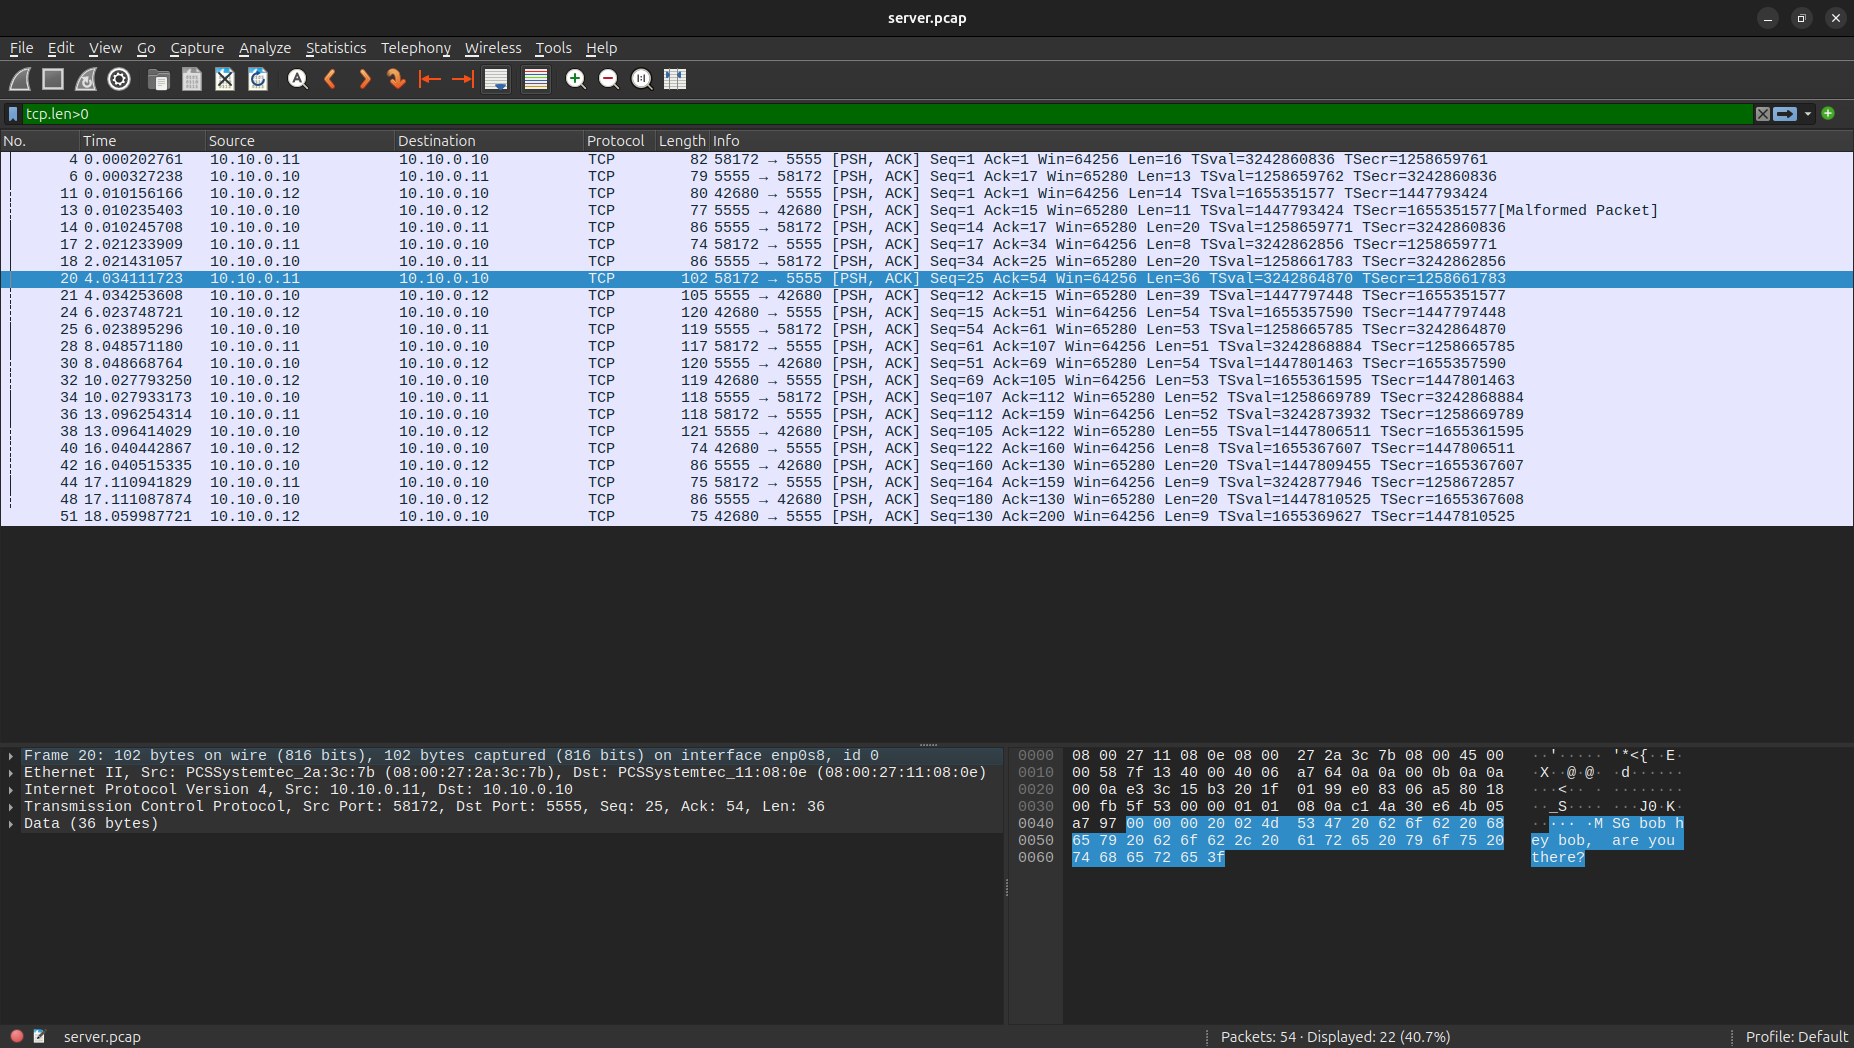
\includegraphics[width=\textwidth]{wireshark-packet-list.png}
\caption{\texttt{server.pcap} opened in Wireshark, filtered to \texttt{tcp.len>0}. Frame~20 is
selected: the bytes pane shows the payload \texttt{MSG bob hey bob, are you there?} directly
readable in ASCII. The preceding five bytes are the record header --- the 4-byte length prefix
\texttt{00 00 00 20} (32 = 1 type byte + 31 payload bytes) followed by the type byte \texttt{02}.}
\label{fig:packets}
\end{figure}

\begin{figure}[htbp]
\centering

\includegraphics[width=\textwidth]{wireshark-follow-tcp-stream.png}
\caption{Follow $\rightarrow$ TCP Stream on \texttt{server.pcap}, stream~0 (client C1 $\leftrightarrow$
server). The entire conversation is legible with no key and no decryption step: the login exchange,
the user list, and every chat message in both directions. Client-to-server data is shown in red,
server-to-client in blue.}
\label{fig:follow}
\end{figure}

\clearpage

The stream contents reproduce as:

\begin{lstlisting}
.....LOGIN alice...      .OK alice.....INFO bob joined.....WHO.....USERS alice bob...
.MSG bob hey bob, are you there?...1.FROM bob yes alice, receiving you loud and clear
.../.MSG bob this line goes to the selected partner...0.FROM bob the server can read
every word of this...0.MSG bob plaintext is fully readable on the wire.....QUIT
\end{lstlisting}

The non-printable characters rendered as dots between messages are the framing itself --- the
four-byte length prefix and the one-byte record type --- so the capture confirms both that the
content is exposed and that the framing behaves as specified.

Anyone with access to the network segment reads the entire conversation, including the usernames.
This is the baseline that the next phase must destroy: repeating this identical capture after adding
confidentiality must show unreadable data at the same offsets.

\subsection{Evidence index}

All files are in \texttt{evidence/phase1/}.

\begin{center}
\small
\begin{tabular}{@{}ll@{}}
\toprule
\textbf{File} & \textbf{Contents} \\
\midrule
\texttt{server.pcap} & Capture on \texttt{vm1-server} (54 packets, both client connections) \\
\texttt{c1.pcap}     & Capture on \texttt{vm2-client1} (27 packets) \\
\texttt{c2.pcap}     & Capture on \texttt{vm3-client2} (27 packets) \\
\texttt{server.log}  & Server relay log with full message content \\
\texttt{wireshark-packet-list.png}        & Wireshark packet view, plaintext in the bytes pane \\
\texttt{wireshark-follow-tcp-stream.png}  & Follow $\rightarrow$ TCP Stream, whole conversation \\
\bottomrule
\end{tabular}
\end{center}

\subsection{Deliverables checklist}

\begin{center}
\small
\begin{tabular}{@{}lc@{}}
\toprule
\textbf{Requirement} & \textbf{Status} \\
\midrule
One server and two clients connected simultaneously over TCP & Done \\
Messages delivered C1 $\rightarrow$ C2 and C2 $\rightarrow$ C1 via the server & Done \\
Server relays each message as-is, without encryption & Done \\
Command interface \texttt{@user}, \texttt{/chat}, \texttt{/who}, \texttt{/quit} & Done \\
Server logs every relayed message; can read full content & Done \\
Wireshark capture with Follow $\rightarrow$ TCP Stream showing plaintext & Done \\
Protocol description: framing, message completeness, routing & Done \\
\bottomrule
\end{tabular}
\end{center}

%======================================================================
\section{Phase 2 --- Confidentiality via Diffie--Hellman}

\begin{keybox}
\textbf{What changed since Phase 1.} A Diffie--Hellman handshake now runs before any application data,
and every record after it is encrypted with AES-256-GCM; the login itself travels encrypted. The
record framing, the \texttt{LOGIN}/\texttt{MSG}/\texttt{WHO} grammar, and the server's routing are
\emph{unchanged} --- the server simply decrypts inbound records and re-encrypts outbound ones. A
man-in-the-middle proxy is added to attack the result.
\end{keybox}

\subsection{Requirements}

Phase~2 requires a Diffie--Hellman key exchange implemented from first principles (a standard
published group, with the modular exponentiation written by hand --- no library DH), an AES key
derived from the shared secret by hashing rather than using it raw, authenticated encryption on all
traffic, a printed fingerprint of the secret on both ends, and a demonstration that the traffic is no
longer readable and that tampering is detected. It also requires a separate man-in-the-middle proxy
that performs two independent exchanges and reads everything.

\subsection{Diffie--Hellman from first principles}

The group is RFC~3526 group~14: a standard, published 2048-bit MODP group with generator $g = 2$,
whose modulus is a safe prime (both $p$ and $(p-1)/2$ are prime). Each side picks a 256-bit private
exponent $x$ and sends $g^{x} \bmod p$; each then computes the shared secret $Z = (\text{peer})^{x}
\bmod p$.

The modular exponentiation is written by hand as \emph{square-and-multiply}, reducing modulo $p$ at
every step. Reducing at each step is not an optimisation but a necessity: with a 2048-bit modulus and
a 256-bit exponent, computing $g^{x}$ before reducing would require an integer with more digits than
there are atoms in the observable universe. OpenSSL's big-integer type is used only as an arithmetic
primitive (\texttt{BN\_mod\_mul}); \texttt{BN\_mod\_exp} and the entire DH API are deliberately
avoided, as the assignment requires. A received public value is rejected unless $1 < y < p-1$, which
prevents a peer from forcing the secret to a value it chooses. A self-test (\texttt{selftest.txt})
confirms the group is a 2048-bit safe prime and that the hand-written exponentiation agrees with
OpenSSL's reference on a range of inputs.

\subsection{Why the shared secret is hashed}

The raw secret $Z$ is \emph{not} used as the AES key. $Z$ is a 2048-bit element of a mathematical
group: its size is wrong for AES-256 (which needs exactly 32 bytes), and its bits are not uniformly
distributed --- some values are structurally more likely, and there are known relationships among the
bits of a modular-exponentiation result. Keying AES with such biased material is unsound. A
cryptographic hash fixes both problems at once: SHA-256 outputs exactly 32 bytes and maps the biased
input to an output indistinguishable from random. Hashing also lets a label and the handshake
transcript be folded in, so the single secret yields several independent values that cannot be
confused with or derived from one another:
\begin{center}\small\ttfamily
K\_c2s = SHA256("CS6008-P2-KEY|c2s|" $\Vert$ Z $\Vert$ TH), \quad
K\_s2c = SHA256("...|s2c|" ...), \quad
FP = SHA256("CS6008-P2-FP|" ...)[0..7]
\end{center}
The two directional keys prevent a record the server sent from being replayed back at it as though the
client had sent it. The fingerprint \texttt{FP} uses a \emph{different} label from the keys, so it can
be printed safely; the raw secret and the keys themselves are never printed.

\subsection{Record encryption}

After the handshake, each \texttt{REC\_APPDATA} body is $\text{ciphertext} \Vert \text{tag}$ under
AES-256-GCM. Neither an IV nor a sequence number is transmitted: the nonce is
$\text{salt}(4) \Vert \text{seq}(8)$ where \texttt{seq} is an implicit per-direction counter each side
maintains independently. TCP delivers records in order, so the counters stay in lockstep; any drop,
duplication, reorder, or injection desynchronises them, the tag fails, and the connection aborts. A
monotonic counter also guarantees the nonce never repeats under one key, which GCM requires.

\subsection{Verification}

\paragraph{Matching fingerprints, secret never printed.} Each client prints the fingerprint of its
derived secret, and it equals the one the server logs for that connection; the two clients differ, as
each runs its own exchange (\texttt{chat-transcript.md}):

\begin{lstlisting}
alice(C1) | key exchange complete, shared-secret fingerprint f5b73958da76b903
SERVER    | KEX ... fingerprint=f5b73958da76b903     <- matches alice
bob(C2)   | key exchange complete, shared-secret fingerprint ef643199d65ce813
SERVER    | KEX ... fingerprint=ef643199d65ce813     <- matches bob
\end{lstlisting}

\paragraph{Traffic is unreadable.} The Phase~1 capture was repeated on the encrypted protocol
(\texttt{chat.pcap}). Every chat word from the session was searched across all frames and found in
none. Figure~\ref{fig:p2packet} shows a chat record's bytes as AES-GCM ciphertext where Phase~1
(Figure~\ref{fig:packets}) showed readable ASCII; Figure~\ref{fig:p2follow} shows Follow $\rightarrow$ TCP
Stream unreadable where Phase~1 (Figure~\ref{fig:follow}) showed the whole conversation.

\begin{figure}[htbp]
\centering
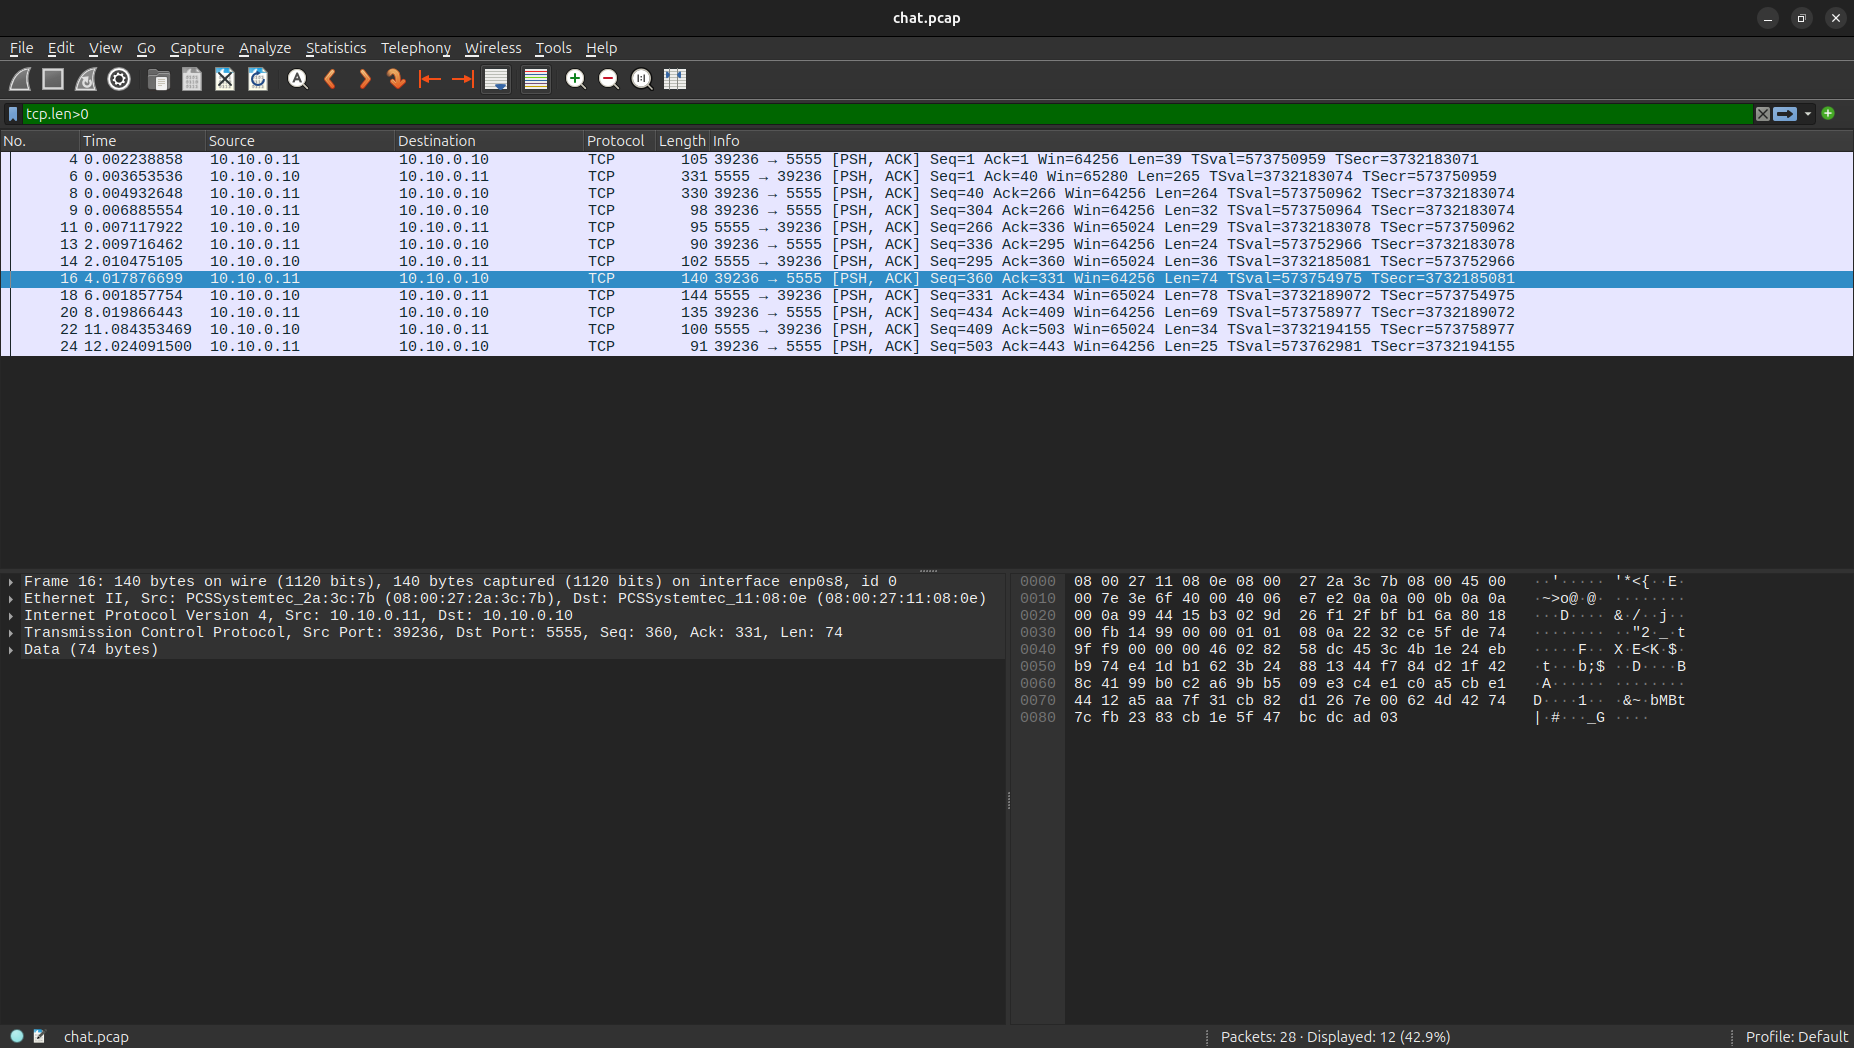
\includegraphics[width=\textwidth]{wireshark-packet-ciphertext.png}
\caption{Phase 2, \texttt{chat.pcap}, frame 16 (a chat record). The bytes pane is AES-GCM ciphertext
with an unreadable ASCII column --- contrast Figure~\ref{fig:packets}, the same view in Phase 1
showing \texttt{MSG bob hey bob, are you there?} in cleartext.}
\label{fig:p2packet}
\end{figure}

\begin{figure}[htbp]
\centering

\includegraphics[width=\textwidth]{wireshark-follow-tcp-stream.png}
\caption{Phase 2, Follow~$\rightarrow$~TCP Stream. Client data in red, server in blue --- all
unreadable, except the two Diffie--Hellman public values (which are meant to be public). Contrast
Figure~\ref{fig:follow}, the same view in Phase 1 with every line legible.}
\label{fig:p2follow}
\end{figure}

\paragraph{Tampering is rejected.} With the proxy's \texttt{-{}-tamper} flag flipping one byte of a
chat record, the login (untampered) is accepted but the corrupted record fails its GCM tag; the server
logs the message \texttt{AES-GCM authentication failed} and closes the connection
(\texttt{tamper-transcript.md}). A single flipped byte is a hard failure, never silent corruption.

\subsection{Attack --- man-in-the-middle}

Diffie--Hellman agrees a key with whoever answers the connection; it never checks who that is. The
proxy (\texttt{mitm.cpp}) exploits this: pointed at by the victim, it runs one exchange as the server
toward the victim and a second as a client toward the real server, holding both keys.

\begin{lstlisting}
victim  <-- DH: session V -->  MALLORY  <-- DH: session S -->  real server
\end{lstlisting}

With \texttt{alice} pointed at the proxy (\texttt{./client 10.10.0.13 alice}) and \texttt{bob} at the
real server, Mallory read and logged every message in plaintext while alice's client reported a normal,
completed, encrypted session (\texttt{mitm-transcript.md}):

\begin{lstlisting}
MALLORY | two sessions established -- victim-side fp=cfbb2a3e...  server-side fp=6d7bdab0...
MALLORY | [C->S] MSG bob this channel feels private to us
MALLORY | [C->S] MSG bob mallory is reading every word
\end{lstlisting}

\paragraph{Detectable evidence, and why a user misses it.} The evidence is the fingerprints. Alice
computed \texttt{cfbb2a3e...} for her session with Mallory, while the real server computed
\texttt{6d7bdab0...} for its session with Mallory --- two different secrets. Had alice and bob compared
fingerprints over an independent channel, the mismatch would have exposed that neither was talking
directly to the other. An ordinary user misses this because unauthenticated Diffie--Hellman gives no
automatic signal: both ends see a normal handshake and a working encrypted session, and the only tell
is a manual, out-of-band comparison that users never perform. This is exactly the gap Phase~3 closes.

\subsection{Deliverables checklist}

\begin{center}
\small
\begin{tabular}{@{}lc@{}}
\toprule
\textbf{Requirement} & \textbf{Status} \\
\midrule
DH from scratch, standard published group, hand-written modular exponentiation & Done \\
AES key derived from the DH secret by hashing, not used raw & Done \\
Authenticated encryption (AES-GCM) on all traffic, login included & Done \\
Both ends print matching fingerprints; raw secret/key never printed & Done \\
Wireshark shows the traffic is no longer readable (before/after) & Done \\
Tampering with a ciphertext byte is rejected, not silently accepted & Done \\
MITM proxy with two independent DH exchanges reads all traffic & Done \\
Explanation: detectable evidence of the MITM and why a user misses it & Done \\
\bottomrule
\end{tabular}
\end{center}

%======================================================================
\section{Building and Running}

\begin{lstlisting}
cd phaseN && make            # phase1: server, client. phase2: + mitm, selftest
make test                    # phase2: run the crypto self-test

# on vm1-server (10.10.0.10)
./server --log server.log

# on vm2-client1 / vm3-client2
./client 10.10.0.10 alice
./client 10.10.0.10 bob

# phase 2 MITM: on vm4-mallory, then point the victim at 10.10.0.13
./mitm --listen 10.10.0.13 --server 10.10.0.10 --log mallory.log [--tamper]

# packet capture, on any VM
sudo tshark -i enp0s8 -f 'tcp port 5555' -w /tmp/cap.pcap
\end{lstlisting}

Two environment notes recorded while capturing: \texttt{dumpcap} drops privileges even when invoked
through \texttt{sudo}, so \texttt{tshark -w} cannot write into a home directory and must target a
world-writable path; and Ubuntu's AppArmor profile prevents \texttt{tshark -r} from reading capture
files stored under \texttt{/home}.

%======================================================================
\section{Next Phase}

Phase~2 established confidentiality but not authentication: the man-in-the-middle attack succeeds
because Diffie--Hellman agrees a key with whoever answers. Phase~3 adds a Public Key Infrastructure ---
a Certificate Authority, a server certificate, and a proof that the server holds the matching private
key --- so the client can verify it is talking to the real server before the exchange proceeds. The
same MITM proxy will then be re-run to show it can no longer succeed.

%======================================================================
\appendix
\section{Generative AI Usage}

As required by assignment section 1.5, every prompt used during this assignment is recorded in

\begin{center}
\ttfamily docs/ai-prompts.md
\end{center}

\noindent
in the submitted repository. The file is maintained incrementally alongside the work rather than
reconstructed afterwards: entries are added in the commit that contains the work they relate to, so
the git history shows the prompts accumulating phase by phase. It is organised by phase, and each
entry records the prompt together with what came out of it.

At the time of writing it covers Phase~0 (lab infrastructure, SSH access, network configuration,
tooling and documentation) and Phase~1 (protocol design, implementation, evidence collection and this
report). It will continue to grow as the remaining phases are implemented.

\end{document}
